\documentclass{webofc}
\usepackage[varg]{txfonts}   % Web of Conferences font
%
% Put here some packages required or/and some personnal commands
%
%
\begin{document}
%
\title{IPv6 in production: its deployment and usage in WLCG}
%
% subtitle is optionnal
%
%%%\subtitle{Do you have a subtitle?\\ If so, write it here}

\author{
  \firstname{Marian} \lastname{Babik}\inst{1}\and
  \firstname{Martin} \lastname{Bly}\inst{2}\and
  \firstname{Tim} \lastname{Chown}\inst{3}\and
  \firstname{Ji\v{r}i} \lastname{Chudoba}\inst{4}\and
  \firstname{Catalin} \lastname{Condurache}\inst{2}\and
  \firstname{Alastair} \lastname{Dewhurst}\inst{2}\and
  \firstname{Xavier} \lastname{Espinal Curull}\inst{1}\and
  \firstname{Thomas} \lastname{Finnern}\inst{5}\and
  \firstname{Terry} \lastname{Froy}\inst{6}\and
  \firstname{Costin} \lastname{Grigoras}\inst{1}\and
  \firstname{Kashif} \lastname{Hafeez}\inst{2}\and
  \firstname{Bruno} \lastname{Hoeft}\inst{7}\and
  \firstname{Hironori} \lastname{Ito}\inst{8}\and
  \firstname{David P.} \lastname{Kelsey}\inst{2}\thanks{\email{david.kelsey@stfc.ac.uk}} \and
  \firstname{Fernando} \lastname{L\'opez~Mu\~noz}\inst{9,10}\fnsep\and
  \firstname{Edoardo} \lastname{Martelli}\inst{1}\and
  \firstname{Raja} \lastname{Nandakumar}\inst{2}\and
  \firstname{Kars} \lastname{Ohrenberg}\inst{5}\and
  \firstname{Francesco} \lastname{Prelz}\inst{11}\and
  \firstname{Duncan} \lastname{Rand}\inst{12}\and
  \firstname{Andrea} \lastname{Sciab\`a}\inst{1}\and
  \firstname{Ulf} \lastname{Tigerstedt}\inst{13}\and
  \firstname{Dennis} \lastname{Van Dok}\inst{14}
}

\institute{ 
  European Organization for Nuclear Research (CERN), CH-1211 Geneva 23, Switzerland
\and
  STFC Rutherford Appleton Laboratory, Harwell Campus, Didcot, Oxfordshire OX11 0QX, United Kingdom
\and
  JISC, Lumen House, Library Avenue, Harwell Campus, Didcot, Oxfordshire OX11 0SG, United Kingdom
\and
  Institute of Physics, Academy of Sciences of the Czech Republic, Na Slovance 2 182 21 Prague 8, Czech Republic
\and
  Deutsches Elektronen-Synchrotron DESY, Notkestra\ss e 85, D-22607 Hamburg, Germany
\and
  Queen Mary University of London, Mile End Road, London E1 4NS, United Kingdom
\and
  Karlsruher Institut f\"ur Technologie, Hermann-von-Helmholtz-Platz 1, D-76344 Eggenstein-Leopoldshafen, Germany 
\and
  Brookhaven National Laboratory, Upton, NY 11973-5000, U.S.A.
\and
  Port d'Informaci\'o Cient\'ifica, Campus UAB, Edifici D, E-08193 Bellaterra, Spain
\and
  Centro de Investigaciones Energ\'eticas, Medioambientales y Tecnol\'ogicas (CIEMAT), Madrid, Spain
\and
  INFN, Sezione di Milano, via G. Celoria 16, I-20133 Milano, Italy
\and
  Imperial College London, South Kensington Campus, London SW7 2AZ, United Kingdom
\and
  Helsinki Institute of Physics, Gustaf H\"allstri\"omin katu 2, FI-00014 Helsinki, Finland
\and
  Nikhef, Science Park 105, NL-1098 XG Amsterdam, The Netherlands. 
          }

\abstract{%
  The fraction of general internet traffic carried over IPv6 continues to 
  grow rapidly. The transition of WLCG central and storage services to 
  dual-stack IPv4/IPv6 is progressing well, thus enabling the use of IPv6-only
  CPU resources as agreed by the WLCG Management Board and presented by us at 
  CHEP2016. By April 2018, all WLCG Tier 1 data centres should provide access to
  their services over IPv6. The LHC experiments have requested all WLCG Tier 2
  centres to provide dual-stack access to their storage by the end of LHC Run 2.
}
%
\maketitle
%
\section{Introduction}
\label{sec-intro}
%section 1

The HEPiX IPv6 Working Group \cite{ipv6wg} has been investigating the many issues involved in the deployment and use of
IPv6 in HEP in general and more specifically in WLCG. The group's paper at CHEP2016 \cite{ipv6chep2016}
presented the status then of the work to allow sites to deploy IPv6-only CPU resources. Driven by the
requirements of the LHC experiments, the WLCG Management Board, in September 2016, had approved our plan
that all WLCG Tier-2 storage services should aim to support dual-stack IPv6/IPv4 by the end of 2018. Since then the
group has worked with others to encourage, support and monitor that transition and to identify and help
solve any technical issues as they arise.

%This paper is organised as follows.  Section 2 presents the current status of the transition for the Tier0/Tier1s, the Tier2s and the Experiment Services.
%Section 3 presents an update on service availability and network monitoring and also reports on the fraction of FTS data transfers currently taking place over IPv6.
%Finally section 4 contains future plans and conclusions. 

 


\section{Status of the transition}
\label{sec-transition-status}
%section 2 Status of the transition to dual-stack storage
% sub-section a) Tier 0 and Tier 1's  (Bruno)
% sub-section b) Tier 2's  (Andrea)
% sub-section c) LHCOPN & LHCONE  (Bruno)
% sub-section d) WLCG Data Transfers (Dave)

% Do we start with a few general words of introduction about the general aims and history of the transition to dual-stack storage?
% Together with reminders of the agreed timetable (and refer to old CHEP papers from our group)?

The long process of enabling the protocol IPv6 at LHC started already 10 years ago in 2010. Today, after extensive testing by the HEPiX IPv6 working group and the strong support of the storage developer community, the current WLCG storage and grid-middleware applications now fully support the use of IPv4 and IPv6 protocols simultaneously; they are dual-stack ready or even protocol agnostic.


% Subsection '2a'
% Tier 0 and Tier 1's
%
%\subsection{Deployment at the Tier-0 and Tier-1 sites}
\subsection{Deployment at Tier-0 and Tier-1's}
After the aforementioned ten years the storage environment is almost completely dual-stack ready. At the CERN WLCG Tier-0 and at the 14 Tier-1s, dual-stack IPv6/IPv4 is nearly fully enabled. Only the Tier-1 site at the Kurchatov Institute in Moscow, part of the Russian Federation, is still currently running on IPv4-only. This enables a total of 96\% of the Tier-1 storage of WLCG to be accessible via IPv6 as shown in table~\ref{tab:t012stor}.
\begin{table}[h]
\centering
\caption{Fraction of Tier-1 and Tier-2 storage available over IPv6}
\label{tab:t012stor}
\begin{tabular}{lccccc}
\hline
& ALICE & ATLAS & CMS & LHCb & Global \\\hline
Tier-1 storage & 78\% & 96\% & 100\% & 94\% & 96\% \\
Tier-2 storage & 86\% & 59\% &  89\% & 75\% & 74\% \\\hline
\end{tabular}
\end{table}

The FTS server at FNAL is still currently running in IPv4 preferred mode. There was a long-standing malfunctioned transfer issue to IPv4-only Tier-2 sites in the USA which is now solved. This last server will be deployed in dual-stack in the near future.

\subsection{Deployment at Tier-2 sites}
The deployment of IPv6 at Tier-2 sites is still proceeding even after the
official deadline expired at the end of 2018. It was decided not to
give the deadline a formal extension, but just to encourage all
remaining sites to complete the IPv6 deployment ``as soon as
possible'': the main motivations were that \emph{a)} sites behind
schedule were encountering objective difficulties and \emph{b)} the
most effective deadline would be imposed by the experiments
themselves, if they wished, for example, to require IPv6 for
production. This choice was confirmed by the steady progress observed
during 2019, as it can be seen in figure~\ref{fig:t2depl}.
\begin{figure}[h]
\centering
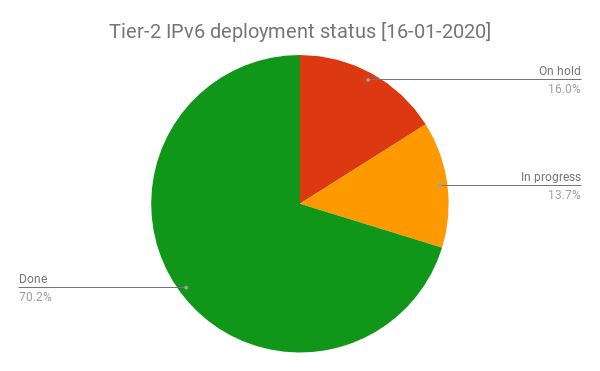
\includegraphics[width=6cm]{chart2}
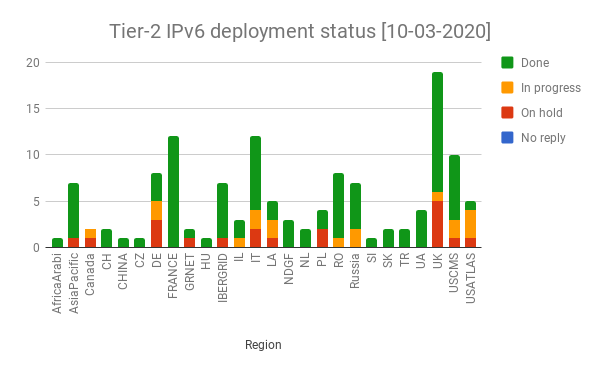
\includegraphics[width=6cm]{chart}
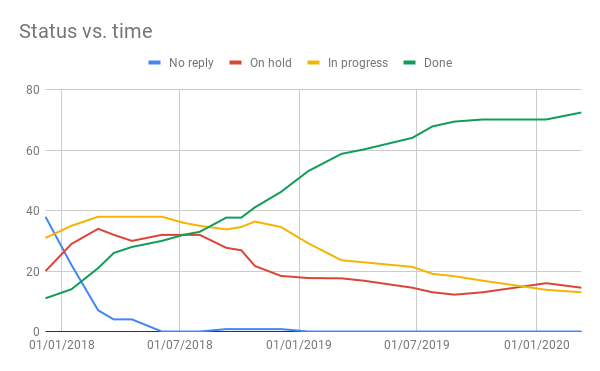
\includegraphics[width=6cm]{chart3}
\caption{(left) Tier-2 deployment status by site globally, (right) by region, and (bottom) time evolution}
\label{fig:t2depl}
\end{figure}

The time evolution of the site status shows a steady increase of the
number of sites that have deployed IPv6, until a more recent
slowdown. This is consistent with the hypothesis that the remaining
sites are those facing the biggest difficulties. A detailed analysis
of the tickets shows that, in many cases, sites need to wait for the
IPv6 deployment on site, which often depends on people different from
the WLCG site staff. The fraction of the Tier-2 storage that is
accessible via IPv6 is shown in table~\ref{tab:t12stor} for each
experiment, and significant differences are apparent.
\begin{table}[h]
\centering
\caption{Fraction of Tier-1 and Tier-2 storage available over IPv6}
\label{tab:t12stor}
\begin{tabular}{lccccc}
\hline
& ALICE & ATLAS & CMS & LHCb & Global \\\hline
Tier-1 storage & 78\% & 96\% & 100\% & 94\% & 96\% \\ 
Tier-2 storage & 86\% & 59\% &  89\% & 75\% & 74\% \\\hline
\end{tabular}
\end{table}
Two experiments (ALICE and CMS) are very close to having all their
Tier-2 storage on IPv6, LHCb has little Tier-2 storage to begin with
due to their particular computing model and ATLAS is getting better,
but still far from the goal.


\subsection{LHCOPN and LHCONE}

The LHCOPN and LHCONE are both virtual private networks (VPN) serving the Large Hadron Colider Experiments. Both networks are from the end of 2016 onward dual-stack ready. LHCOPN is a CERN (Tier-0) centric star network mainly deployed for the distribution of the raw detector data to the Tier-1 sites. Since the majority of Tier-1 sites are dual-stack ready and even while the protocol IPv6 is preferred it is still not the situation that IPv6 is the only transfer protocol, but a tendency towards IPv6 file transfers are recognizable. LHCONE is a network of close to 140 sites connected trough Virtual Routing and Forwarding implementations at 26 different network service providers (NSP). All connected end sites deploying a Border Gateway Protocol (BGP) routing table and advertising their own Classless Inter-Domain Routing (CIDR) to the connecting NSP. The network itself is already since long IPv6 ready. The connected end sites are becoming more and more IPv6 ready. This is recognizable at the  transfer protocol changes from IPv4 towards IPv6. The high usage of the IPv4 transfer protocol visualizes that the fraction of IPv4 only sites is still quite substantial.

%section{File Transfers

\subsection{File transfers}

Over the last 2 years we have been regularly tracking the fraction of WLCG file transfers that take place over IPv6.
(needs more description).

The fraction of data transfers over FTS on IPv6 as a function of date is shown in  figure~\ref{fig:FTS}.
\begin{figure}[h]
\centering
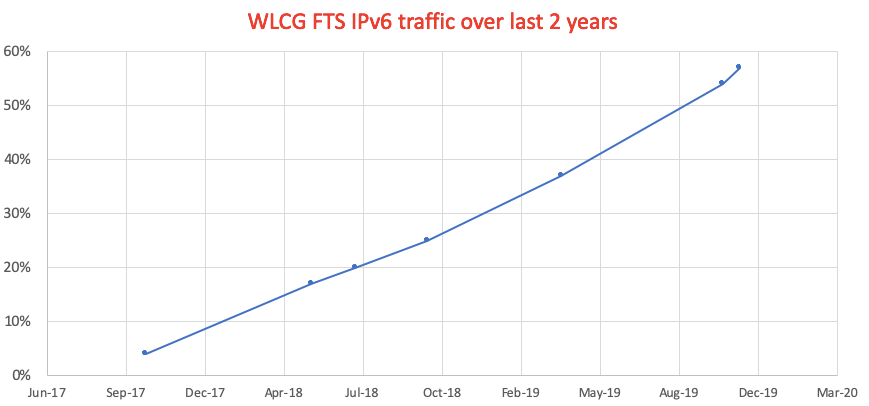
\includegraphics[width=10cm]{FTS}
\caption{Percentage of FTS data transfers over IPv6}
\label{fig:FTS}
\end{figure}


%% Subsection '2a'
% Tier 0 and Tier 1's
%
Some efforts were made to investigate whether the WLCG software packages could be enabled to run in a dual-stack environment or even become protocol agnostic. The first software packages that were examined were data transfer software packages like FTS and SRM. After the examination some software packages were replaced like AFS with EOS, or CASTOR with DPM. Today the storage environment is dual/stack ready and at CERN the Tier-0 is IPv6 and IPv4 dual-stack is enabled. The Tier-1 sites: CA-Triumf, DE-KIT, ES-PIC, FR-CCIN2P3, IT-INFN-CNAF, NDGF, NL-T1 (SARA-Matrix and NIKHEF), RRC-JINR-T1, TW-ASGC, UK-T1-RAL, US-T1-BNL, US-T1-FNAL are dual-stack deployed as shown in the following figure. ~\ref{fig:t1ds}.
\begin{figure}[t]
\centering
%\includegraphics[width=13cm]{Tier-1-IPv6-dual-stack}
\includegraphics[width=13cm]hepix-ipv6-tier01-dual-stack.png}
%\includegraphics[width=13cm]{t1ds}
\caption{Tier-0/1 IPv4/6 dual-stack redyness incl dual-stack perfsonar server deployment}
\label{fig:t1ds}
\end{figure}

But even while the IPv6 redeaness deadline in April 2018 is long ago, there is one part of the russian Tier-1 RRC-KI-T1 still deployed with IPv4 only. The dual-stack perfsonar server is deployed at almost all sites except NL-T1-NIKHEF and RRC-KI-T1. The FTS server at FNAL is still running in IPv4 prefered mode. There were a long standing malfunctioned transfer issue to IPv4 only US-Tier-2 sites which is solved now. This last server will get deployed in dual-stack as soon as possible.   

%\subsection{Deployment at Tier-2 sites}
The deployment of IPv6 at Tier-2 sites is still proceeding even after the
official deadline expired at the end of 2018. It was decided not to
give the deadline a formal extension, but just to encourage all
remaining sites to complete the IPv6 deployment ``as soon as
possible'': the main motivations were that \emph{a)} sites behind
schedule were encountering objective difficulties and \emph{b)} the
most effective deadline would be imposed by the experiments
themselves, if they wished, for example, to require IPv6 for
production. This choice was confirmed by the steady progress observed
during 2019, as it can be seen in figure~\ref{fig:t2depl}.
\begin{figure}[h]
\centering
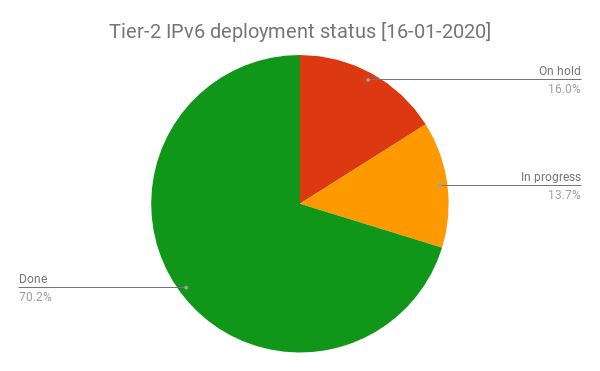
\includegraphics[width=6cm]{chart2}
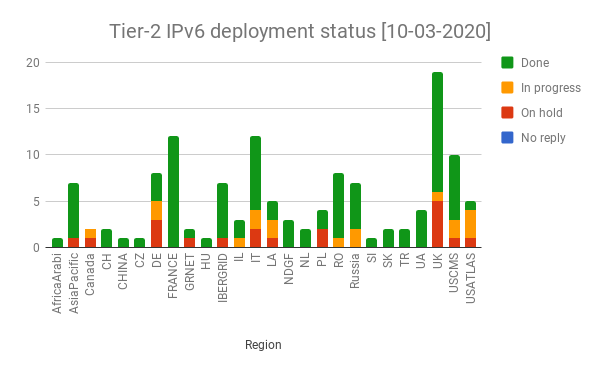
\includegraphics[width=6cm]{chart}
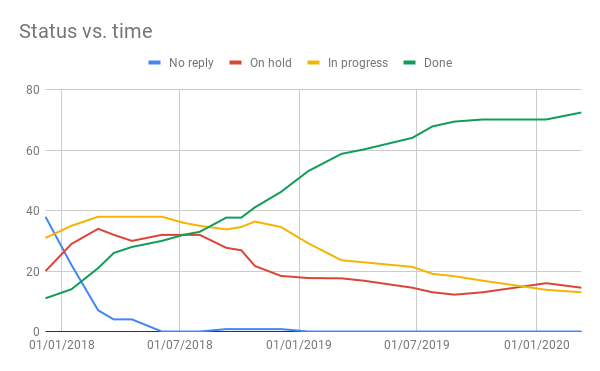
\includegraphics[width=6cm]{chart3}
\caption{(left) Tier-2 deployment status by site globally, (right) by region, and (bottom) time evolution}
\label{fig:t2depl}
\end{figure}

The time evolution of the site status shows a steady increase of the
number of sites that have deployed IPv6, until a more recent
slowdown. This is consistent with the hypothesis that the remaining
sites are those facing the biggest difficulties. A detailed analysis
of the tickets shows that, in many cases, sites need to wait for the
IPv6 deployment on site, which often depends on people different from
the WLCG site staff. The fraction of the Tier-2 storage that is
accessible via IPv6 is shown in table~\ref{tab:t12stor} for each
experiment, and significant differences are apparent.
\begin{table}[h]
\centering
\caption{Fraction of Tier-1 and Tier-2 storage available over IPv6}
\label{tab:t12stor}
\begin{tabular}{lccccc}
\hline
& ALICE & ATLAS & CMS & LHCb & Global \\\hline
Tier-1 storage & 78\% & 96\% & 100\% & 94\% & 96\% \\ 
Tier-2 storage & 86\% & 59\% &  89\% & 75\% & 74\% \\\hline
\end{tabular}
\end{table}
Two experiments (ALICE and CMS) are very close to having all their
Tier-2 storage on IPv6, LHCb has little Tier-2 storage to begin with
due to their particular computing model and ATLAS is getting better,
but still far from the goal.


%\subsection{LHCOPN and LHCONE}

The LHCOPN and LHCONE are both virtual private networks (VPN) serving the Large Hadron Colider Experiments. Both networks are from the end of 2016 onward dual-stack ready. LHCOPN is a CERN (Tier-0) centric star network mainly deployed for the distribution of the raw detector data to the Tier-1 sites. Since the majority of Tier-1 sites are dual-stack ready and even while the protocol IPv6 is preferred it is still not the situation that IPv6 is the only transfer protocol, but a tendency towards IPv6 file transfers are recognizable. LHCONE is a network of close to 140 sites connected trough Virtual Routing and Forwarding implementations at 26 different network service providers (NSP). All connected end sites deploying a Border Gateway Protocol (BGP) routing table and advertising their own Classless Inter-Domain Routing (CIDR) to the connecting NSP. The network itself is already since long IPv6 ready. The connected end sites are becoming more and more IPv6 ready. This is recognizable at the  transfer protocol changes from IPv4 towards IPv6. The high usage of the IPv4 transfer protocol visualizes that the fraction of IPv4 only sites is still quite substantial.




\section{Monitoring}
\label{sec-monitoring}
%section 3

\subsection{SAM}
WLCG Service Availability Monitoring (SAM) \cite{sam} has been one of the primary tools to track and report on availability and reliability of the WLCG sites. The monthly generated reports are based on profiles, which define how exactly a specific set of metrics are aggregated and which site services are taken into account, for example, a sample profile would usually require at least one computing element at the site to be able to accept and run jobs and all storage elements to pass basic write/list/read tests on a sample file. 

The underlying measurement tool that provides the metrics to SAM is WLCG Experiments Test Framework (ETF) \cite{etf}. ETF provides low level monitoring framework used to test core sites services at regular intervals, performing basic "ping-like" tests on remote compute, worker nodes and storage. A separate dual-stack ETF infrastructure has been setup during 2017 and runs alongside the production IPv4-only infrastructure. Running two separate ETF clusters, IPv4-only and dual-stack, is primarily intended to help sites easily identify problems with their IPv6 migration by comparing results of the exact same tests run over the two different protocols.  Additional testing and debugging was also performed to migrate ETF dual-stack infrastructure into IPv6-only in order to ensure that the production testing would not fallback to the IPv4 while at the same time facilitate the evaluation of the dependent services such as myproxy, os/middleware repositories, time servers, configuration and orchestration environments (Puppet/OpenStack), etc. 

In February 2018, ETF dual-stack infrastructure became production ready and started publishing its results to SAM. The final step in the migration process was to understand how to define profiles that would mix both IPv4 and IPv6 results and this was achieved by introducing a separate IPv4 and IPv6 service types that can be used in the aggregation algorithm to combine the results coming from ETF. This means that each site service can now be identified with corresponding IPv4 and IPv6 type, which in turn makes it possible to define profiles that would require a site to have either IPv4 or IPv6 computing element while requiring its storage to be both IPv4 and IPv6 capable. This feature is currently offered in pre-production and is available to the experiments for evaluation. Once evaluated and deployed to production, it will make it possible for SAM to generate the WLCG monthly availability and reliability reports for both IPv4 and/or IPv6 depending on the profile setup by the experiments. 

\subsection{perfSONAR}
The WLCG has adopted the perfSONAR toolkit \cite{perfsonar} for the monitoring of its network infrastructure and its deployment and configuration is being coordinated by the WLCG Network Throughput working group \cite{wlcg-NTWG}.  perfSONAR offers a very good way of checking that the migration to IPv6 hasn't caused any network/routing issues as it clearly separates IPv4 and IPv6 network measurements while supporting full range of network testing including throughput, latency, packet loss, packet re-ordering and duplicates, network path and packet retransmits.

Testing within WLCG is organised by a central configuration system (PWA), which operates around groups of sites also referred to as meshes. Currently, there are meshes for each  experiment such as ATLAS, CMS and LHCb as well as network groupings such as LHCONE and LHCOPN and since 2017 a dedicated dual-stack mesh was introduced, which groups together all dual-stack hosts on the network. Following the working group campaign to deploy dual-stack services at all Tier-1s and Tier-2s, the number of dual-stack hosts has grown to cover almost 50\% of the infrastructure, currently there are 132 dual-stack perfSONARs out of total 268 available. In collaboration with GEANT, additional dual-stack perfSONARs were deployed at their major network hubs in London, Paris, Amsterdam, Geneva and Frankfurt, which has greatly facilitated debugging of potential routing and performance issues. 

Successful adoption rate of dual-stack perfSONAR has lead to a proposal in late 2017 to integrate IPv6 testing directly into the existing production meshes, which would significantly improve the test coverage and eventually bring it on par with IPv4. This migration is currently in progress and was already implemented for LHCOPN, LHCONE, USATLAS, USCMS and ATLAS. Tests currently being migrated include network throughput, packet re-transmits, network path and round-trip time, which together provide a very good testing core to identify and locate potential network routing and performance issues. As latency and packet loss testing for IPv6 would require significant resources, doubling the current testing capacity which is already at its limits, it was proposed that a dedicated dual-stack mesh will be kept for now. 

In addition to the configuration changes, there has been also good progress in the area of visualisation. Recently, new Grafana-based dashboard has been deployed to complement the existing Maddash \cite{psmad} and a dedicated IPv6 view was setup \cite{grafana-ipv6} to help sites compare side-by-side their IPv4 and IPv6 perfSONAR measurements. This view is still a work in progress, but once all meshes are migrated and the overall test coverage improves, it will offer an important operational overview of the status of IPv6 network performance. 

\subsection{FTS}
%In the WLCG bulk data transport is carried out predominantly by the File Transfer Service (FTS3)  \cite{638647551}. The monitoring data reported by each FTS3 server for such data transfers indicate whether IPv6 was used during the transfer. Figure~\ref{fig:fts} (top) shows FTS data transfers \cite{grafana-FTS} for all VOs (not just the WLCG experiments) over 30 days in September-October 2018. It can be seen that whilst IPv4 still dominates IPv6 is used approximately a quarter of the time. Interestingly, transfers over IPv6 appear to be more reliable (figure~\ref{fig:fts} bottom), hovering around the 95\% mark whilst transfers over IPv4 average approximately 75\% success rate. It is speculated that this is because the sites which have implemented IPv6 first tend to be the more reliable ones. In order for FTS transfers to go over IPv6 both of the storage elements and the FTS server itself need to be dual-stack. Currently, of the eight FTS servers in regular use by the WLCG, five are dual-stack. It is planned that at least one of the remaining three will enable IPv6 at the end of LHC Run 2.

In WLCG bulk data transport is carried out predominantly by the File Transfer Service (FTS3)  \cite{638647551}. The monitoring data reported by each FTS3 server for such data transfers indicate whether IPv6 was used during the transfer. Figure~\ref{fig:fts} shows FTS data transfers \cite{grafana-FTS} for all VOs (not just the WLCG experiments) during the month of October 2018. It can be seen that whilst IPv4 still dominates IPv6 is used approximately a quarter of the time. Interestingly, transfers over IPv6 appear to be more reliable, hovering around the 95\% mark whilst transfers over IPv4 average approximately 75\% success rate. It is speculated that this is because the sites which have implemented IPv6 first tend to be the more reliable ones. In order for FTS transfers to go over IPv6 both of the storage elements and the FTS server itself need to be dual-stack. Currently, of the eight FTS servers in regular use by the WLCG, five are dual-stack. It is planned that at least one of the remaining three will enable IPv6 at the end of LHC Run 2.

\begin{figure}[t]
\centering
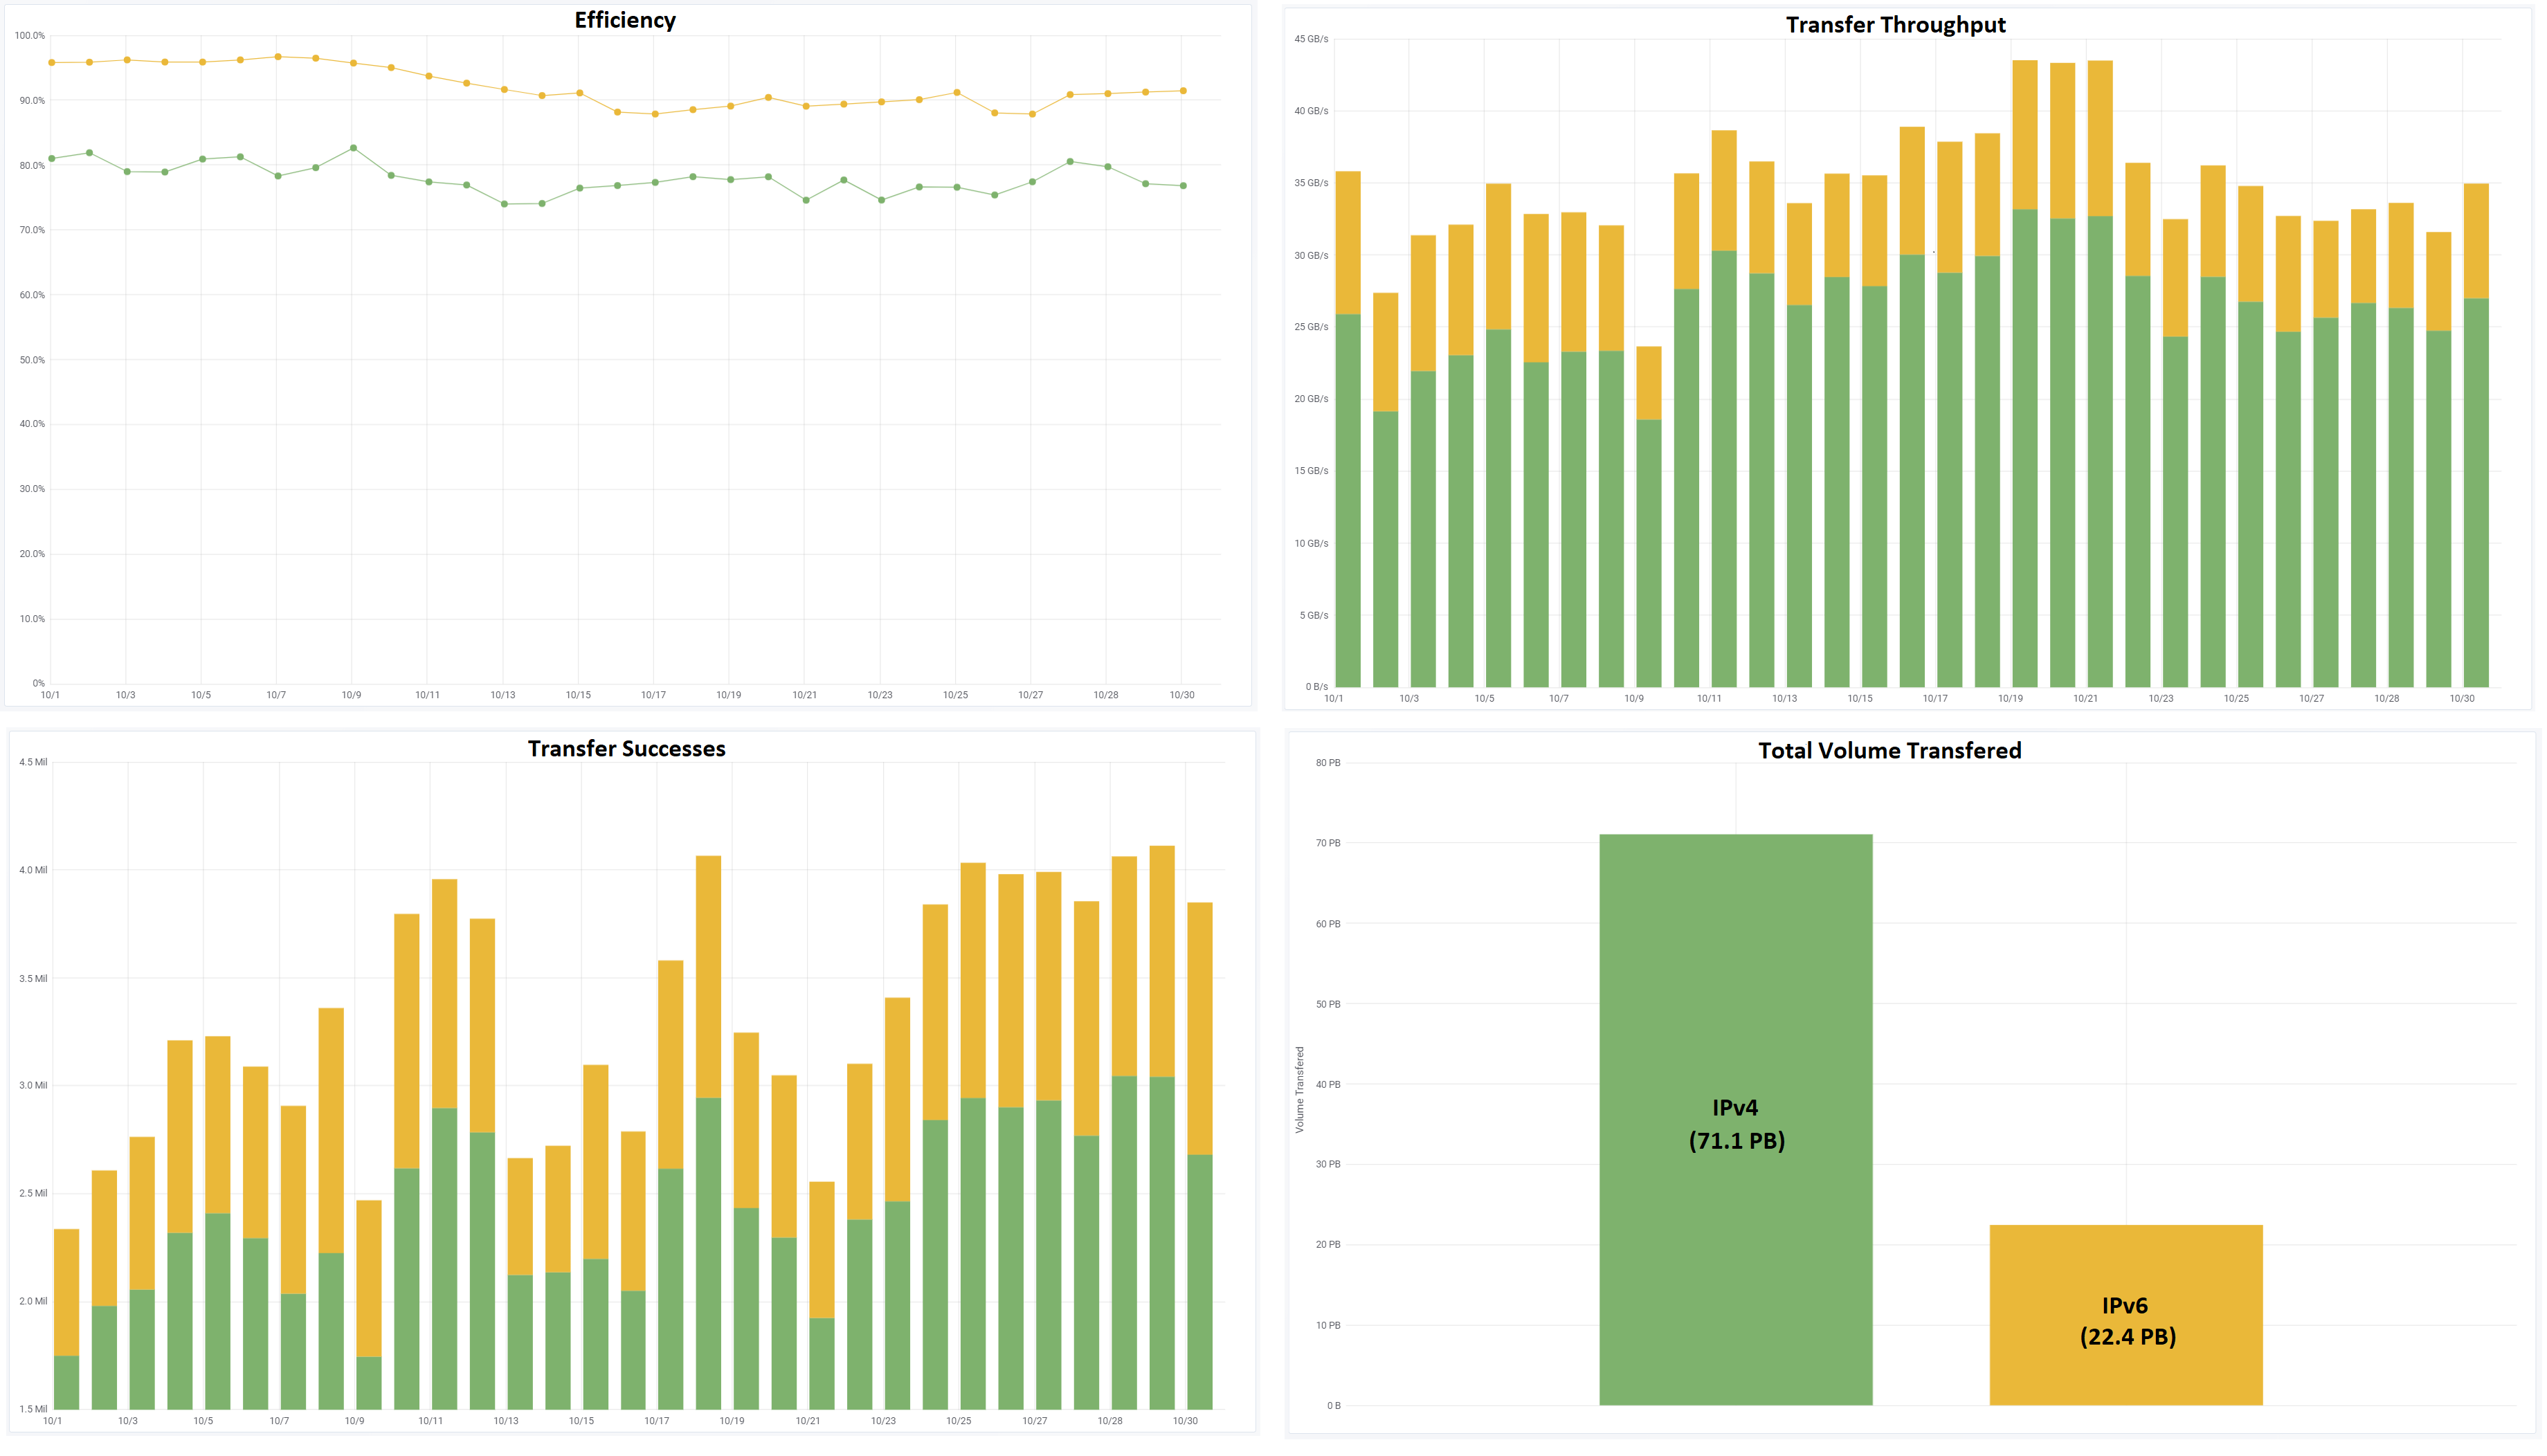
\includegraphics[width=13cm]{FTS-IPv6-figure}
%\includegraphics[width=13cm]{fts1}
%\includegraphics[width=13cm]{fts2}
\caption{FTS transfer throughput for Oct 2018 and success rate according to whether IPv6 was used. IPv4 is green; IPv6 is amber}
\label{fig:fts}
\end{figure}

\subsection{XrootD}
The other major method by which data is accessed, often remotely, is XrootD most notably by the ALICE and CMS experiments. Currently, the Monit WLCG Transfers Monitoring Service at CERN \cite{grafana-WLCG-Transfers} does not display whether this data was transferred over IPv4 or IPv6. However, the XrootD monitoring data has now been updated to report whether IPv4 or IPv6 was used \cite{xrootd-ipv6} and work is in progress to include this information in the Monit monitoring.




\section{Future plans and conclusions}
\label{sec-future}
%section 4
\subsection{Obstacles and potential show-stoppers}
Our experience with the transition of WLCG Tier-1 and Tier-2 centers so far 
has identified various cases where the IPv4$\rightarrow$IPv6 transition has
consequences that exceed the simple replacement of the IP {\it transport} layer.
These broadly fall in the following categories:
\begin{enumerate}
\item Software components and protocol with fixed-size storage for network
addresses, for example in (Grid-)FTP and AFS. This can be overcome by appropriate
protocol extensions (e.g. the introduction of 'extended' FTP commands
{\tt EPRT}, {\tt EPSV}, etc.), with a large development effort required.
In certain cases (AFS) this effort was determined to be too large and not
worthwhile, while the GrifFTP 'v2' extensions were issued with no IPv6 support.
\item Software components and protocols that assume single addresses or a single
IP protocol for 
network endpoints (to various extents, all the components in the WLCG software
matrix). While all Operating Systems do provide hybrid network stacks and prioritized/configurable
source and destination address selection\footnote{Address selection is regulated in most cases by RFC6724.}, applications should always iterate over multiple
possible results (belonging to multiple IP protocol versions) and provide configurable
overrides and preferences. 
\item Software components and network infrastructures providing asymmetric
handling, or separate code stacks, for IPv4 and IPv6 traffic: these also
have the ability to load the network transport choice with measurable
performance consequences.
\end{enumerate}
Detecting and explaining these IPv4/IPv6 asymmetries and fostering improved
symmetry across the WLCG software matrix has been a long-standing activity
for our group. As there is inherent risk in changing, testing and rolling
out (sometimes sizable) software changes when no functional
issue requires immediate attention, these changes are often not shortlisted
for deployment by software development teams. We need to continue tracking
these issues down to the
level where no deployment of measurable performance asymmetry between the two
protocols is seen: this can be seen as the backdrop of any future activity.

\subsection{Further steps}
Once the data transfer monitoring infrastructure described in Section
\ref{sec-monitoring} is completed and covers all services, two cases
need to be consistently monitored and, where needed, investigated
and resolved:
\begin{enumerate}
\item cases where the fraction of data transferred over IPv6 is lower than expected:
the preference for IPv6 over IPv4 has to established throughout the system;
\item cases where the transfer performance is either significantly worse 
or significantly better on IPv6 over IPv4: asymmetries in the routing and
transport should be identified, especially in the LHCONE and LHCOPN networks.
\end{enumerate}
\par
Over a stable and understood data transfer network 
IPv6-only worker nodes should encounter no more operational anomalies
than other types of worker nodes. The 
job failure rate on IPV6-only, dual-stack and IPv4-only worker nodes should
be monitored statistically and deviations properly troubleshot.
\par
Once the use-case of IPv6-only worker nodes operates smoothly, the next
step in the transition roadmap is moving services and network segments to
IPv6-only operation.

\subsection{IPv6-only scenarios}
The final step of the IPv4$\rightarrow$IPv6 transition is the phasing out of
IPv4. While still in the non-near future, this is also arguably the only step
that can bring along a desirable reduction
in the infrastructure maintenance effort, so it shouldn't be delayed
without reason. Many of the issues described in the previous sections 
actually arise
from the fact that in the current transition phase many components and
configurations have to be maintained in parallel.
\par
In order to demonstrate that the close of the transition is a realistic
objective, IPv6-only operation of an entire WLCG Tier-X site will
need to have been proven by all experiments and sites run by most WLCG
partners, with residual IPv4-only services either deprecated or made
accessible via protocol translation techniques (e.g. DNS64/NAT64, see
NAT64/DNS64 (RFC6146/6147 \cite{rfc})). 
\par
%{\it XXX Should we mention the few experiments performed so far here ?}

\subsection{Conclusion}
The aim of allowing the successful execution of generic WLCG job payloads
on IPv6-only worker nodes has been driving the IPv4-IPv6 dual-stack deployment
of storage services across the WLCG production infrastructure. According to
the current progress tracking, summarised in Sections \ref{ssec-t1trans} and
\ref{ssec-t2trans} above, this step should be completed at CERN, Tier-1
and Tier-2 centres by the end of 2018. A few residual
issues were identified in the software stack in this process.
\par
Data from
a complete and pervasive monitoring infrastructure are crucial in building
confidence in the new transport layer, which is expected to provide the
{\it same} level of performance and reliability as the one it replaces: these
come from various sources (see Section \ref{sec-monitoring}), with a few
remaining blind spots being covered.
\par
Feedback from the actual operation of  
IPv6-only computing farms will then determine the time-scale and viability of
driving the transition process to its natural ending, when the burden
of operating a duplicated transport infrastructure will be eventually lifted.



%For one-column wide figures use syntax of figure~\ref{fig-1}
%\begin{figure}[h]
%% Use the relevant command for your figure-insertion program
%% to insert the figure file.
%\centering
%\includegraphics[width=1cm,clip]{tiger}
%\caption{Please write your figure caption here}
%\label{fig-1}       % Give a unique label
%\end{figure}
%
%For two-column wide figures use syntax of figure~\ref{fig-2}
%\begin{figure*}
%\centering
%% Use the relevant command for your figure-insertion program
%% to insert the figure file. See example above.
%% If not, use
%\vspace*{5cm}       % Give the correct figure height in cm
%\caption{Please write your figure caption here}
%\label{fig-2}       % Give a unique label
%\end{figure*}
%
%For figure with sidecaption legend use syntax of figure
%\begin{figure}
%% Use the relevant command for your figure-insertion program
%% to insert the figure file.
%\centering
%\sidecaption
%\includegraphics[width=5cm,clip]{tiger}
%\caption{Please write your figure caption here}
%\label{fig-3}       % Give a unique label
%\end{figure}
%
%For tables use syntax in table~\ref{tab-1}.
%\begin{table}
%\centering
%\caption{Please write your table caption here}
%\label{tab-1}       % Give a unique label
%% For LaTeX tables you can use
%\begin{tabular}{lll}
%\hline
%first & second & third  \\\hline
%number & number & number \\
%number & number & number \\\hline
%\end{tabular}
%% Or use
%\vspace*{5cm}  % with the correct table height
%\end{table}
%
% BibTeX or Biber users please use (the style is already called in the class, ensure that the "woc.bst" style is in your local directory)
% \bibliography{name or your bibliography database}
%
% Non-BibTeX users please use
%
\begin{thebibliography}{}
%
% and use \bibitem to create references.
%
\bibitem{rfc} All Internet Engineering Task Force Requests For Comments (RFC) do
cuments are available
from URLs such as http://www.ietf.org/rfc/rfcNNNN.txt where NNNN is the RFC numb
er, for example {\tt http://www.ietf.org/rfc/rfc2460.txt}
% Format for Journal Reference
Journal Author, Journal \textbf{Volume}, page numbers (year)
% Format for books
\bibitem{RefB}
Book Author, \textit{Book title} (Publisher, place, year) page numbers
% etc
\end{thebibliography}

\end{document}

% end of file template.tex

<div id='footer'><table width='100%'><tr><td class='right'><a href='http://fusioninventory.org/'><span class='copyright'>FusionInventory 9.1+1.0 | copyleft <img src='/glpi/plugins/fusioninventory/pics/copyleft.png'/>  2010-2016 by FusionInventory Team</span></a></td></tr></table></div>
